\documentclass[aspectratio=169]{beamer}

% ---------- ENCODING & FONTS ----------
\usepackage[utf8]{inputenc}
\usepackage[T1]{fontenc}

% ---------- THEME & LOOK ----------
\usetheme{Madrid}
\usecolortheme{seahorse}
\usefonttheme{professionalfonts}
\setbeamertemplate{navigation symbols}{}
\setbeamercovered{transparent}
\setbeamertemplate{itemize items}[circle]
\setbeamertemplate{enumerate items}[default]
\setlength{\parskip}{0.25em}

% ---------- COLORS ----------
\definecolor{accent}{RGB}{0,92,184}
\definecolor{soft}{RGB}{233,244,255}
\definecolor{canadared}{RGB}{196,30,58}
\definecolor{leafgreen}{RGB}{0,130,80}
\definecolor{goldenrod}{RGB}{218,165,32}
\definecolor{deeporange}{RGB}{220,90,20}
\definecolor{shiftpurple}{RGB}{130,50,180}
\definecolor{tealblue}{RGB}{0,128,128}
\definecolor{lightred}{RGB}{245,210,210}
\setbeamercolor{structure}{fg=accent}
\setbeamercolor{title}{fg=white,bg=accent}
\setbeamercolor{frametitle}{fg=accent}
\setbeamercolor{block title}{bg=accent!12,fg=accent}
\setbeamercolor{block body}{bg=soft}

% ---------- PACKAGES ----------
\usepackage{booktabs}
\usepackage{amsmath, amssymb}
\usepackage{array}
\usepackage{multirow}
\usepackage{hyperref}
\usepackage{tikz}
\usepackage{pgfplots}
\pgfplotsset{compat=1.18}
\usetikzlibrary{arrows.meta, positioning, calc, shapes.geometric, patterns}
\hypersetup{colorlinks=true,linkcolor=accent,urlcolor=accent}

% ---------- SAFE TRANSITION FALLBACK ----------
\makeatletter
\@ifundefined{transfade}{\newcommand{\transfade}[1][]{}}{}
\makeatother

% ---------- TITLE ----------
\title{\textbf{Economic Growth, the Financial System, and Business Cycles}}
\subtitle{{\large ECON 101 -- Principles of Macroeconomics}}
\author{Muhebullah Karimzada}
\date{Spring 2026}

% ============================================================
\begin{document}
% ============================================================

\begin{frame}[plain]
  \titlepage
\end{frame}

\begin{frame}{Chapter Outline}
\transfade
\begin{itemize}[<+->]
  \item \textbf{6.1} Long-Run Economic Growth
  \item \textbf{6.2} Saving, Investment, and the Financial System
  \item \textbf{6.3} The Business Cycle
\end{itemize}
\end{frame}

% ============================================================
\section{6.1 Long-Run Economic Growth}
% ============================================================

\begin{frame}{6.1 Learning Objective}
\transfade
\begin{block}{Goal}
Explain how long-run economic growth is measured and what determines it.
\end{block}
\begin{itemize}[<+->]
  \item \textbf{Long-run economic growth:} the process by which rising \alert{productivity} increases the \textbf{average standard of living}.
  \item This differs from short-run fluctuations (\textbf{business cycles}):
  \begin{itemize}[<+->]
    \item \textbf{Expansion:} real GDP rising.
    \item \textbf{Recession:} real GDP falling.
  \end{itemize}
  \item The most common measure of the standard of living:
  \begin{itemize}[<+->]
    \item \textbf{Real GDP per capita} $=$ real GDP $\div$ population.
  \end{itemize}
\end{itemize}
\end{frame}

\begin{frame}{Real GDP per Capita: A Key Indicator}
\transfade
\begin{itemize}[<+->]
  \item \textbf{Real GDP per capita} tells us:
  \begin{itemize}[<+->]
    \item How much goods and services, on average, each person can consume.
    \item Adjusted for changes in the price level (\textbf{real}, not nominal).
  \end{itemize}
  \item Countries with higher real GDP per capita typically have:
  \begin{itemize}[<+->]
    \item better health, education, housing, and infrastructure.
  \end{itemize}
  \item \textbf{Canadian context:} In 2023, Canada's real GDP per capita was approximately \alert{\$53,000} (2012 constant dollars), roughly \textbf{four times} the 1961 level of $\approx$\$13,800.
  \begin{itemize}[<+->]
    \item \textcolor{goldenrod}{Source: Statistics Canada, Table 36-10-0222-01}
  \end{itemize}
\end{itemize}
\end{frame}

\begin{frame}{Figure 6.1 -- Real GDP per Capita in Canada, Selected Years}
\begin{center}
\begin{tikzpicture}
\begin{axis}[
  width=0.85\textwidth, height=0.72\textheight,
  ybar, bar width=0.55cm,
  xlabel={Year},
  ylabel={Real GDP per Capita (2012 \$000s)},
  symbolic x coords={1961,1971,1981,1991,2001,2011,2019,2023},
  xtick=data,
  ymin=0, ymax=60,
  enlarge x limits=0.08,
  nodes near coords,
  nodes near coords style={font=\tiny, color=black},
  every axis plot/.append style={fill=accent!70, draw=accent},
  grid=major, grid style={dotted, gray!50},
  tick label style={font=\small},
  label style={font=\small},
  title style={font=\small\bfseries},
  title={Canada's Real GDP per Capita Has Quadrupled Since 1961}
]
\addplot coordinates {(1961,13.8)(1971,19.5)(1981,25.8)(1991,29.0)(2001,37.8)(2011,46.5)(2019,51.8)(2023,53.2)};
\end{axis}
\end{tikzpicture}
\end{center}
{\tiny Source: Statistics Canada, Table 36-10-0222-01 (2012 constant dollars).}
\end{frame}

\begin{frame}{Interpretation of Figure 6.1}
\transfade
\begin{itemize}[<+->]
  \item Measured in 2012 dollars, real GDP per capita has risen \textbf{nearly four-fold} since 1961.
  \item The average Canadian in 2023 commands \alert{almost four times as many} goods and services as the average Canadian in 1961.
  \item This long-run rise is what we call \textbf{economic growth}.
  \item \textbf{Notable interruptions:}
  \begin{itemize}[<+->]
    \item Early 1980s recession (high interest rates, oil price shock).
    \item Early 1990s recession (tight monetary policy, housing bust).
    \item 2008--2009 Global Financial Crisis.
    \item \alert{2020 COVID-19 pandemic}: real GDP per capita fell $\approx$13\% in just 2 quarters --- the sharpest decline on record.
  \end{itemize}
\end{itemize}
\end{frame}

% ------------------------------------------------------------
% Growth Rates & Rule of 70
% ------------------------------------------------------------

\begin{frame}{Calculating Growth Rates}
\transfade
\begin{itemize}[<+->]
  \item Growth rate of an economic variable from year $t-1$ to year $t$:
  \[
    \text{Growth rate}_t = \frac{\text{Value}_t - \text{Value}_{t-1}}{\text{Value}_{t-1}} \times 100.
  \]
  \item For a few years, compute growth each year and take the average.
  \item \textbf{Canadian example:}
  \begin{itemize}[<+->]
    \item Real GDP per capita in 2022: \$53,100.
    \item Real GDP per capita in 2023: \$53,200.
    \item Growth rate $\approx \dfrac{53{,}200 - 53{,}100}{53{,}100} \times 100 \approx \textbf{0.19\%}$.
    \item \textcolor{canadared}{Canada's 2023 growth was very weak --- immigration drove population faster than real output.}
  \end{itemize}
\end{itemize}
\end{frame}

\begin{frame}{The Rule of 70}
\transfade
\begin{itemize}[<+->]
  \item A handy shortcut: the \textbf{Rule of 70}.
  \item If a variable grows at rate $g$\% per year, the number of years to \textbf{double} is approximately:
  \[
    \text{Years to double} \approx \frac{70}{g}.
  \]
  \item \textbf{Canadian examples:}
  \begin{itemize}[<+->]
    \item Canada's historical average growth of real GDP per capita $\approx 2\%$:
    \item Years to double $\approx 70 / 2 = \alert{35}$ years.
    \item At only 1\% growth: $70 / 1 = \alert{70}$ years --- twice as long!
  \end{itemize}
  \item Small differences in growth rates \textbf{compound} dramatically over decades.
\end{itemize}
\end{frame}

\begin{frame}{Rule of 70: Country Comparison}
\transfade
\begin{columns}
\column{0.48\textwidth}
\begin{block}{Country A --- 2\% growth}
\begin{itemize}
  \item Years to double: $70/2 = 35$
  \item Income after 35 years: \textbf{2x}
  \item Income after 70 years: \textbf{4x}
\end{itemize}
\end{block}
\column{0.48\textwidth}
\begin{block}{Country B --- 4\% growth}
\begin{itemize}
  \item Years to double: $70/4 = 17.5$
  \item Income after 35 years: \textbf{4x}
  \item Income after 70 years: \textbf{16x}
\end{itemize}
\end{block}
\end{columns}
\vspace{0.5em}
\begin{itemize}[<+->]
  \item \textbf{Real example:} South Korea's economy grew $\approx 7\%$ per year from 1960 to 2000, doubling every 10 years --- raising per capita income from $\approx$\$1{,}000 to $\approx$\$20{,}000 (2000 US\$).
  \item Canada's steadier $\approx 2\%$ average represents \textcolor{leafgreen}{sustained prosperity without boom-and-bust volatility}.
\end{itemize}
\end{frame}

% ------------------------------------------------------------
% What Determines Long-Run Growth?
% ------------------------------------------------------------

\begin{frame}{What Determines Long-Run Growth?}
\transfade
\begin{itemize}[<+->]
  \item Long-run increases in real GDP per capita depend on \textbf{labour productivity}:
  \[
    \text{Labour productivity} = \frac{\text{Real GDP}}{\text{Number of workers (or hours worked)}}.
  \]
  \item The average Canadian produces much more per hour than in 1961.
  \item Two key drivers:
  \begin{enumerate}[<+->]
    \item \textbf{Increases in capital per hour worked}
    \item \textbf{Technological change}
  \end{enumerate}
  \item \textbf{Canadian data (Statistics Canada):} Labour productivity grew an average of \alert{1.4\%} per year from 2000--2023 --- slower than the G7 average, raising policy concern.
\end{itemize}
\end{frame}

\begin{frame}{Capital per Hour Worked}
\transfade
\begin{itemize}[<+->]
  \item \textbf{Physical capital:} machines, computers, tools, buildings, vehicles.
  \begin{itemize}[<+->]
    \item More capital per worker $\Rightarrow$ more output per hour.
  \end{itemize}
  \item \textbf{Human capital:}
  \begin{itemize}[<+->]
    \item Accumulated knowledge and skills from education, training, experience.
  \end{itemize}
  \item \textbf{Canadian example:}
  \begin{itemize}[<+->]
    \item A Canadian oil sands worker equipped with modern extraction technology and earth-moving equipment produces orders of magnitude more output per day than a 1961 worker with manual tools.
    \item BC's tech sector: engineers with university degrees and high-powered workstations represent both physical and human capital investment.
  \end{itemize}
\end{itemize}
\end{frame}

\begin{frame}{Technological Change}
\transfade
\begin{itemize}[<+->]
  \item \textbf{Technological change:} improvements in methods of combining inputs into outputs.
  \item Examples:
  \begin{itemize}[<+->]
    \item New production processes (AI-assisted manufacturing).
    \item Better management (lean production, just-in-time inventory).
    \item New products (mRNA vaccines, electric vehicles).
  \end{itemize}
  \item Workers produce more \textbf{with the same inputs} --- an outward shift of the production frontier.
  \item \textbf{Canadian example:} Shopify (Ottawa) enables thousands of small businesses to reach global markets with the same team size --- a pure technology-driven productivity gain.
  \item \textbf{Entrepreneurs} pioneer these new ways of combining labour, capital, and ideas.
\end{itemize}
\end{frame}

% ------------------------------------------------------------
% Potential GDP & Output Gap
% ------------------------------------------------------------

\begin{frame}{Potential GDP}
\transfade
\begin{itemize}[<+->]
  \item \textbf{Potential GDP:} the level of real GDP attained when all firms produce at \textbf{capacity} ---
  \begin{itemize}[<+->]
    \item ``normal'' hours, ``normal'' workforce, no emergency overtime.
  \end{itemize}
  \item Also called \textbf{full-employment GDP} or \textbf{trend GDP}.
  \item Potential GDP grows when:
  \begin{itemize}[<+->]
    \item the labour force expands (e.g., through immigration),
    \item new factories and equipment are installed,
    \item technological change raises productivity.
  \end{itemize}
  \item \textbf{Bank of Canada} estimates and monitors potential GDP as part of its quarterly Monetary Policy Report (MPR).
\end{itemize}
\end{frame}

\begin{frame}{Figure 6.2 -- Output Gap: Canada 2015--2025 (Estimated)}
\begin{center}
\begin{tikzpicture}
\begin{axis}[
  width=0.88\textwidth, height=0.70\textheight,
  xlabel={Year},
  ylabel={Output Gap (\% of Potential GDP)},
  xmin=2015, xmax=2025.5,
  ymin=-14, ymax=5,
  xtick={2015,2016,2017,2018,2019,2020,2021,2022,2023,2024,2025},
  xticklabel style={rotate=45, anchor=east, font=\tiny},
  ytick={-14,-12,-10,-8,-6,-4,-2,0,2,4},
  grid=both, grid style={dotted,gray!40},
  tick label style={font=\tiny},
  label style={font=\small},
  title style={font=\small\bfseries},
  title={Canada's Output Gap Swung Sharply During COVID-19}
]
% Actual output gap data (approximate, Bank of Canada estimates)
\addplot[accent, very thick, mark=*, mark size=1.5pt] coordinates {
  (2015,-1.0)(2016,-0.8)(2017,-0.5)(2018,0.2)(2019,0.1)
  (2020,-13.0)(2021,-2.5)(2022,1.8)(2023,-0.3)(2024,-1.2)(2025,-0.8)
};
% Zero line
\addplot[black, dashed, thick] coordinates {(2015,0)(2025.5,0)};
\node[font=\tiny, text=black] at (axis cs:2016.5,0.5) {Potential GDP};
% COVID annotation
\node[font=\tiny, align=center, fill=white, draw=canadared, rounded corners]
  at (axis cs:2020.5,-10.5) {COVID-19 Recession};
% 2022 boom annotation
\node[font=\tiny, align=center, fill=white, draw=leafgreen, rounded corners]
  at (axis cs:2022.5,2.8) {Post-Pandemic Boom};
\end{axis}
\end{tikzpicture}
\end{center}
{\tiny Source: Bank of Canada, Monetary Policy Report (estimates). Shaded area = negative output gap (recessionary).}
\end{frame}

\begin{frame}{The Output Gap}
\transfade
\begin{itemize}[<+->]
  \item \textbf{Output gap:} $= $ actual GDP $-$ potential GDP.
  \item When the output gap is \textbf{positive} (actual $>$ potential):
  \begin{itemize}[<+->]
    \item economy is using resources \alert{unsustainably} --- very low unemployment, high capacity utilization, \textbf{inflationary pressure}.
    \item \textbf{Canada 2022}: output gap $\approx +1.8\%$ coincided with CPI inflation peaking at \alert{8.1\%}.
  \end{itemize}
  \item When the output gap is \textbf{negative} (actual $<$ potential):
  \begin{itemize}[<+->]
    \item resources (labour, capital) are \alert{underutilized}.
    \item \textbf{Canada 2020}: output gap plunged to $\approx -13\%$ during COVID-19 lockdowns.
  \end{itemize}
  \item The Bank of Canada uses the output gap to guide its monetary policy decisions (MPR, 2024).
\end{itemize}
\end{frame}

% ============================================================
\section{6.2 Saving, Investment, and the Financial System}
% ============================================================

\begin{frame}{6.2 Learning Objective}
\transfade
\begin{block}{Goal}
Explain how the financial system links saving and investment and why that matters for growth.
\end{block}
\begin{itemize}[<+->]
  \item Long-run growth requires:
  \begin{itemize}[<+->]
    \item more capital per worker, and ongoing technological improvements.
  \end{itemize}
  \item Both require \textbf{investment}.
  \item Investment is financed by \textbf{saving}, channeled through the financial system.
  \item \textbf{Canadian saving rate} (household, \% of disposable income): fell from $\approx$18\% in 1982 to $\approx$2--4\% pre-COVID, then \alert{surged} to 28\% during 2020 lockdowns (Statistics Canada).
\end{itemize}
\end{frame}

\begin{frame}{An Overview of the Financial System}
\transfade
\begin{itemize}[<+->]
  \item \textbf{Financial markets:} where financial securities are bought and sold.
  \begin{itemize}[<+->]
    \item Toronto Stock Exchange (TSX), bond markets, money markets.
  \end{itemize}
  \item \textbf{Stock:} financial security representing partial \textbf{ownership} of a firm.
  \begin{itemize}[<+->]
    \item Buying TSX-listed Shopify shares $\Rightarrow$ you own part of Shopify.
  \end{itemize}
  \item \textbf{Bond:} financial security promising to repay a \textbf{fixed amount} of funds.
  \begin{itemize}[<+->]
    \item Government of Canada bonds, corporate bonds (e.g., TD Bank bonds).
    \item A bond is effectively a \textbf{loan} from the buyer to the issuer.
  \end{itemize}
  \item \textbf{Financial intermediaries:} firms that borrow from savers and lend to borrowers.
  \begin{itemize}[<+->]
    \item Royal Bank, TD, Scotiabank, credit unions, mutual funds, pension funds (e.g., CPPIB).
  \end{itemize}
\end{itemize}
\end{frame}

\begin{frame}{Three Key Services of the Financial System}
\transfade
\begin{columns}
\column{0.32\textwidth}
\begin{block}{\centering \textcolor{accent}{Risk-Sharing}}
\begin{itemize}
  \item Spread money across many assets.
  \item Reduces risk while maintaining returns.
  \item \textit{E.g., RBC Select Balanced mutual fund.}
\end{itemize}
\end{block}
\column{0.32\textwidth}
\begin{block}{\centering \textcolor{leafgreen}{Liquidity}}
\begin{itemize}
  \item Ease of converting to cash.
  \item Bank accounts, money market funds, publicly traded stocks.
  \item Allows long-term commitments with short-term access.
\end{itemize}
\end{block}
\column{0.32\textwidth}
\begin{block}{\centering \textcolor{deeporange}{Information}}
\begin{itemize}
  \item Prices of securities aggregate expectations.
  \item Guide funds toward the most productive uses.
  \item Reduce adverse selection and moral hazard.
\end{itemize}
\end{block}
\end{columns}
\end{frame}

% ------------------------------------------------------------
% Saving and Investment: Macroeconomic Identity
% ------------------------------------------------------------

\begin{frame}{The Macroeconomics of Saving and Investment}
\transfade
\begin{itemize}[<+->]
  \item National income identity:
  \[
    Y = C + I + G + NX.
  \]
  \item For simplicity, assume a \textbf{closed economy} ($NX = 0$):
  \[
    Y = C + I + G \quad \Rightarrow \quad I = Y - C - G.
  \]
  \item Investment equals total income not consumed or used by government.
  \item \textbf{Private saving:}
  \[
    S_{\text{private}} = Y + \text{TR} - C - T.
  \]
  \item \textbf{Public saving:}
  \[
    S_{\text{public}} = T - G - \text{TR}.
  \]
  \item \textbf{Total saving = Investment:}
  \[
    \boxed{S = S_{\text{private}} + S_{\text{public}} = I}
  \]
\end{itemize}
\end{frame}

\begin{frame}{Budget Deficits and Crowding Out}
\transfade
\begin{itemize}[<+->]
  \item If $S_{\text{public}} < 0$: government runs a \textbf{budget deficit}.
  \begin{itemize}[<+->]
    \item Government must borrow (sell bonds), reducing funds available for private investment.
  \end{itemize}
  \item \textbf{Crowding out:} the reduction in private investment caused by government borrowing.
  \item \textbf{Canadian context:}
  \begin{itemize}[<+->]
    \item Federal government ran deficits every year 2009--2024.
    \item 2020--21 deficit: \alert{\$314 billion} (largest ever), due to COVID-19 emergency spending.
    \item 2023--24 deficit: \$40 billion (Department of Finance Canada).
  \end{itemize}
  \item In practice, crowding-out effects on interest rates are partially offset by global capital flows.
\end{itemize}
\end{frame}

% ------------------------------------------------------------
% Market for Loanable Funds
% ------------------------------------------------------------

\begin{frame}{Figure 6.3 -- The Market for Loanable Funds}
\begin{center}
\begin{tikzpicture}
\begin{axis}[
  width=0.72\textwidth, height=0.72\textheight,
  xlabel={Quantity of Loanable Funds (\$ billions)},
  ylabel={Real Interest Rate (\%)},
  xmin=0, xmax=10, ymin=0, ymax=8,
  xtick={0,2,4,6,8,10}, ytick={0,1,2,3,4,5,6,7,8},
  grid=major, grid style={dotted,gray!40},
  tick label style={font=\small},
  label style={font=\small},
  title style={font=\small\bfseries},
  title={Equilibrium in the Loanable Funds Market}
]
% Supply (upward sloping - saving)
\addplot[leafgreen, very thick, domain=0:9] {0.6*x + 0.5}
  node[right, font=\small, color=leafgreen] {\textbf{S} (Saving)};
% Demand (downward sloping - investment)
\addplot[canadared, very thick, domain=0:9] {-0.6*x + 7.7}
  node[right, font=\small, color=canadared] {\textbf{D} (Investment)};
% Equilibrium point
\addplot[accent, only marks, mark=*, mark size=4pt] coordinates {(6.0,4.1)};
\draw[dashed, gray, thick] (axis cs:6.0,4.1) -- (axis cs:6.0,0) node[below, font=\small] {$Q^*=\$600$B};
\draw[dashed, gray, thick] (axis cs:6.0,4.1) -- (axis cs:0,4.1) node[left, font=\small] {$r^*=4\%$};
\node[font=\small, fill=soft, draw=accent, rounded corners, inner sep=2pt, above right]
  at (axis cs:6.0,4.1) {Equilibrium};
\end{axis}
\end{tikzpicture}
\end{center}
\end{frame}

\begin{frame}{Supply and Demand for Loanable Funds}
\transfade
\begin{itemize}[<+->]
  \item \textbf{Demand for loanable funds} (firms):
  \begin{itemize}[<+->]
    \item Firms borrow to finance investment projects.
    \item Borrow more when real interest rate is \textbf{lower} (more projects profitable).
    \item \textbf{Canada 2020}: pandemic uncertainty slashed private investment by $\approx$15\%.
  \end{itemize}
  \item \textbf{Supply of loanable funds} (households):
  \begin{itemize}[<+->]
    \item Households save more when real interest rate is \textbf{higher} (greater reward to saving).
    \item Government saving (surplus) adds to supply; deficits reduce supply.
  \end{itemize}
  \item \textbf{Real interest rate} adjusts to equate saving and investment.
\end{itemize}
\end{frame}

\begin{frame}{Figure 6.4 -- Increase in Demand for Loanable Funds}
\begin{center}
\begin{tikzpicture}
\begin{axis}[
  width=0.72\textwidth, height=0.70\textheight,
  xlabel={Quantity of Loanable Funds},
  ylabel={Real Interest Rate (\%)},
  xmin=0, xmax=10, ymin=0, ymax=8,
  grid=major, grid style={dotted,gray!40},
  tick label style={font=\tiny},
  label style={font=\small},
  title style={font=\small\bfseries},
  title={Tech Boom Raises Demand $\Rightarrow$ Higher $r^*$ and $Q^*$}
]
\addplot[leafgreen, very thick, domain=0:9] {0.6*x + 0.5}
  node[right, font=\tiny, color=leafgreen] {\textbf{S}};
\addplot[canadared!60, very thick, dashed, domain=0:9] {-0.6*x + 7.7}
  node[right, font=\tiny, color=canadared!60] {$D_1$};
\addplot[deeporange, very thick, domain=0:9] {-0.6*x + 9.3}
  node[right, font=\tiny, color=deeporange] {$D_2$ (tech boom)};
\addplot[accent, only marks, mark=*, mark size=3pt] coordinates {(6.0,4.1)};
\addplot[deeporange, only marks, mark=*, mark size=3pt] coordinates {(7.33,4.9)};
\draw[dashed,gray] (axis cs:6,4.1)--(axis cs:6,0) node[below,font=\tiny]{$Q_1$};
\draw[dashed,gray] (axis cs:7.33,4.9)--(axis cs:7.33,0) node[below,font=\tiny]{$Q_2$};
\draw[dashed,gray] (axis cs:6,4.1)--(axis cs:0,4.1) node[left,font=\tiny]{$r_1$};
\draw[dashed,gray] (axis cs:7.33,4.9)--(axis cs:0,4.9) node[left,font=\tiny]{$r_2$};
\draw[->, very thick, shiftpurple] (axis cs:4.5,6.5) -- (axis cs:6.2,6.5)
  node[right, font=\tiny, color=shiftpurple]{Shift};
\end{axis}
\end{tikzpicture}
\end{center}
\end{frame}

\begin{frame}{Figure 6.5 -- Budget Deficit Crowds Out Investment}
\begin{center}
\begin{tikzpicture}
\begin{axis}[
  width=0.72\textwidth, height=0.70\textheight,
  xlabel={Quantity of Loanable Funds},
  ylabel={Real Interest Rate (\%)},
  xmin=0, xmax=10, ymin=0, ymax=8,
  grid=major, grid style={dotted,gray!40},
  tick label style={font=\tiny},
  label style={font=\small},
  title style={font=\small\bfseries},
  title={Government Deficit Reduces Supply $\Rightarrow$ Higher $r^*$, Lower Private $Q^*$}
]
\addplot[canadared, very thick, domain=0:9] {-0.6*x + 7.7}
  node[right, font=\tiny, color=canadared] {\textbf{D}};
\addplot[leafgreen, very thick, domain=0:9] {0.6*x + 0.5}
  node[right, font=\tiny, color=leafgreen] {$S_1$};
\addplot[goldenrod, very thick, domain=0:8.5] {0.6*x + 2.0}
  node[right, font=\tiny, color=goldenrod] {$S_2$ (deficit)};
\addplot[accent, only marks, mark=*, mark size=3pt] coordinates {(6.0,4.1)};
\addplot[goldenrod, only marks, mark=*, mark size=3pt] coordinates {(4.75,4.85)};
\draw[dashed,gray] (axis cs:6,4.1)--(axis cs:6,0) node[below,font=\tiny]{$Q_1$};
\draw[dashed,gray] (axis cs:4.75,4.85)--(axis cs:4.75,0) node[below,font=\tiny]{$Q_2$};
\draw[dashed,gray] (axis cs:6,4.1)--(axis cs:0,4.1) node[left,font=\tiny]{$r_1$};
\draw[dashed,gray] (axis cs:4.75,4.85)--(axis cs:0,4.85) node[left,font=\tiny]{$r_2$};
\draw[->, very thick, canadared] (axis cs:3.5,3.5) -- (axis cs:2.3,3.5)
  node[left, font=\tiny, color=canadared, align=left]{Crowding Out};
\node[font=\tiny, fill=lightred, rounded corners, align=center]
  at (axis cs:5.5,6.5) {Gov't deficit shifts S left $\Rightarrow$ crowding out};
\end{axis}
\end{tikzpicture}
\end{center}
\end{frame}

% ============================================================
\section{6.3 The Business Cycle}
% ============================================================

\begin{frame}{6.3 Learning Objective}
\transfade
\begin{block}{Goal}
Explain what happens during the business cycle and how it affects inflation and unemployment.
\end{block}
\begin{itemize}[<+->]
  \item Real GDP per capita has risen about \textbf{four-fold} since 1961, but not smoothly.
  \item Canada has experienced several recessions:
  \begin{itemize}[<+->]
    \item 1981--82, 1990--91, 2008--09, and \alert{2020}.
  \end{itemize}
  \item The \textbf{business cycle} describes these short-run fluctuations.
\end{itemize}
\end{frame}

\begin{frame}{Figure 6.6 -- Phases of the Business Cycle}
\begin{center}
\begin{tikzpicture}[scale=1.0]
\begin{axis}[
  width=0.88\textwidth, height=0.65\textheight,
  xlabel={Time},
  ylabel={Real GDP},
  xmin=0, xmax=12, ymin=3, ymax=9,
  xtick=\empty, ytick=\empty,
  axis lines=left,
  grid=none,
  label style={font=\small},
  title style={font=\small\bfseries},
  title={The Idealized Business Cycle}
]
% Long-run trend
\addplot[black, dashed, thick, domain=0:12] {0.3*x + 4.5}
  node[right, font=\tiny] {Potential GDP (trend)};
% Actual GDP (sine wave around trend)
\addplot[accent, very thick, smooth, domain=0:12, samples=100]
  {0.3*x + 4.5 + 1.2*sin(deg(1.4*x))};
% Labels for phases
\node[font=\tiny, fill=leafgreen!20, draw=leafgreen, rounded corners] at (axis cs:1.3,6.8) {Expansion};
\node[font=\tiny, fill=canadared!20, draw=canadared, rounded corners] at (axis cs:3.5,4.5) {Recession};
\node[font=\tiny, fill=leafgreen!20, draw=leafgreen, rounded corners] at (axis cs:5.8,7.2) {Expansion};
\node[font=\tiny, fill=canadared!20, draw=canadared, rounded corners] at (axis cs:7.8,4.9) {Recession};
% Peak and trough arrows
\draw[->, goldenrod, thick] (axis cs:2.2,7.4) node[above, font=\tiny, color=goldenrod]{\textbf{Peak}} -- (axis cs:2.2,7.0);
\draw[->, goldenrod, thick] (axis cs:4.4,4.0) node[below, font=\tiny, color=goldenrod]{\textbf{Trough}} -- (axis cs:4.4,4.4);
\draw[->, goldenrod, thick] (axis cs:6.7,7.8) node[above, font=\tiny, color=goldenrod]{\textbf{Peak}} -- (axis cs:6.7,7.4);
\draw[->, goldenrod, thick] (axis cs:8.9,4.5) node[below, font=\tiny, color=goldenrod]{\textbf{Trough}} -- (axis cs:8.9,4.9);
\end{axis}
\end{tikzpicture}
\end{center}
\end{frame}

\begin{frame}{Phases of the Business Cycle}
\transfade
\begin{itemize}[<+->]
  \item \textbf{Expansion:} real GDP is rising (employment grows, incomes rise).
  \item \textbf{Peak:} the point where real GDP stops rising and begins to fall.
  \item \textbf{Recession:} real GDP is falling (often defined as 2+ consecutive quarters).
  \item \textbf{Trough:} the point where real GDP stops falling and begins to rise.
  \item A new expansion follows the trough.
\end{itemize}
\vspace{0.3em}
\begin{block}{Canadian Recessions Since 1980}
\small
\begin{tabular}{lll}
\toprule
\textbf{Recession} & \textbf{Cause} & \textbf{Peak Unemployment} \\
\midrule
1981--82 & Volcker rate shock & 13.0\% \\
1990--91 & Tight monetary policy & 11.9\% \\
2008--09 & Global financial crisis & 8.7\% \\
2020 & COVID-19 pandemic & \alert{14.6\%} (May 2020) \\
\bottomrule
\end{tabular}
\end{block}
{\tiny Source: Statistics Canada, Labour Force Survey.}
\end{frame}

\begin{frame}{How Does Canada Identify Recessions?}
\transfade
\begin{itemize}[<+->]
  \item There is \textbf{no official body} in Canada that declares recessions.
  \item Common rule of thumb:
  \begin{itemize}[<+->]
    \item \textbf{Two consecutive quarters} of negative real GDP growth.
  \end{itemize}
  \item Statistics Canada (CANSIM) provides real GDP data quarterly and monthly.
  \item \textbf{2020 example:}
  \begin{itemize}[<+->]
    \item Q1 2020: real GDP fell $-$8.8\% (annualized).
    \item Q2 2020: real GDP fell $-$38.7\% (annualized) --- deepest quarterly drop on record.
    \item Economy recovered to 2019 levels only by end of 2021.
  \end{itemize}
\end{itemize}
\end{frame}

\begin{frame}{Figure 6.7 -- Inflation and the Business Cycle (Canada)}
\begin{center}
\begin{tikzpicture}
\begin{axis}[
  width=0.88\textwidth, height=0.68\textheight,
  xlabel={Year},
  ylabel={CPI Inflation Rate (\%)},
  xmin=2018, xmax=2025.5,
  ymin=-1, ymax=9,
  xtick={2018,2019,2020,2021,2022,2023,2024,2025},
  xticklabel style={rotate=45, anchor=east, font=\tiny},
  grid=both, grid style={dotted,gray!40},
  tick label style={font=\tiny},
  label style={font=\small},
  title style={font=\small\bfseries},
  title={Canada CPI Inflation Fell in Recession, Surged in Recovery}
]
\addplot[canadared, very thick, mark=square*, mark size=1.5pt] coordinates {
  (2018,2.3)(2019,1.9)(2020,0.7)(2021,3.4)(2022,6.8)(2023,3.9)(2024,2.7)(2025,2.1)
};
\addplot[goldenrod, dashed, thick] coordinates {(2018,2)(2025.5,2)}
  node[right, font=\tiny, color=goldenrod] {BoC Target (2\%)};
\addplot[accent!30, fill=accent!10] coordinates {(2018,2)(2025.5,2)(2025.5,3)(2018,3)} -- cycle;
\node[font=\tiny, fill=lightred, draw=canadared, rounded corners, align=center]
  at (axis cs:2022,7.8) {Peak: 6.8\%\\(June 2022: 8.1\%)};
\node[font=\tiny, fill=white, draw=accent, rounded corners, align=center]
  at (axis cs:2020,1.5) {COVID:\\0.7\%};
\end{axis}
\end{tikzpicture}
\end{center}
{\tiny Source: Statistics Canada, Table 18-10-0004-01. 2025 is estimated. BoC target band 1--3\% shaded.}
\end{frame}

\begin{frame}{The Effect of the Business Cycle on Inflation}
\transfade
\begin{itemize}[<+->]
  \item \textbf{During recessions:}
  \begin{itemize}[<+->]
    \item Demand falls below supply capacity.
    \item Firms compete for fewer customers $\Rightarrow$ prices rise more slowly or fall.
    \item \textbf{Canada 2020}: CPI inflation dropped to \alert{0.7\%}.
  \end{itemize}
  \item \textbf{During expansions:}
  \begin{itemize}[<+->]
    \item Demand exceeds supply capacity.
    \item Firms can raise prices more easily $\Rightarrow$ higher inflation.
    \item \textbf{Canada 2022}: Post-COVID surge in demand + supply chain disruptions $\Rightarrow$ CPI peaked at \alert{8.1\%} in June 2022 (Statistics Canada).
  \end{itemize}
  \item Bank of Canada responded with the \textbf{fastest rate-hike cycle in decades}: 0.25\% $\to$ 5.0\% (March 2022 -- July 2023).
\end{itemize}
\end{frame}

\begin{frame}{Figure 6.8 -- Unemployment and the Business Cycle (Canada)}
\begin{center}
\begin{tikzpicture}
\begin{axis}[
  width=0.88\textwidth, height=0.68\textheight,
  xlabel={Year},
  ylabel={Unemployment Rate (\%)},
  xmin=2018, xmax=2025.5,
  ymin=4, ymax=16,
  xtick={2018,2019,2020,2021,2022,2023,2024,2025},
  xticklabel style={rotate=45, anchor=east, font=\tiny},
  grid=both, grid style={dotted,gray!40},
  tick label style={font=\tiny},
  label style={font=\small},
  title style={font=\small\bfseries},
  title={Unemployment Rose Sharply in 2020, Then Gradually Climbed Again}
]
\addplot[accent, very thick, mark=*, mark size=1.5pt] coordinates {
  (2018,5.8)(2019,5.7)(2020,9.6)(2021,7.5)(2022,5.3)(2023,5.4)(2024,6.3)(2025,6.5)
};
\addplot[leafgreen, dashed, thick] coordinates {(2018,5.5)(2025.5,5.5)}
  node[right, font=\tiny, color=leafgreen] {Est. Natural Rate ($\approx$5.5\%)};
\node[font=\tiny, fill=lightred, draw=canadared, rounded corners, align=center]
  at (axis cs:2020,11.5) {COVID Peak\\14.6\% (May 2020)};
\node[font=\tiny, fill=white, draw=accent, rounded corners]
  at (axis cs:2022.5,4.8) {5.3\%: post-1970s low};
\end{axis}
\end{tikzpicture}
\end{center}
{\tiny Source: Statistics Canada, Labour Force Survey (Table 14-10-0017-01). 2025 is estimated.}
\end{frame}

\begin{frame}{The Effect of the Business Cycle on Unemployment}
\transfade
\begin{itemize}[<+->]
  \item \textbf{During recessions:}
  \begin{itemize}[<+->]
    \item Firms see sales fall, reduce production, lay off workers.
    \item Unemployment often \textbf{continues to rise} even after the recession begins (lagging indicator).
    \item \textbf{Canada 2020}: unemployment hit \alert{14.6\%} in May 2020.
  \end{itemize}
  \item \textbf{During expansions:}
  \begin{itemize}[<+->]
    \item Firms hire more; unemployment gradually falls.
    \item \textbf{Canada 2022}: unemployment reached \alert{5.3\%}, near a 50-year low, amid very tight labour markets.
  \end{itemize}
  \item \textbf{Canada 2023--2024:} rising immigration \& slowing economy pushed unemployment back up to \alert{6.3\%} --- signalling excess slack.
\end{itemize}
\end{frame}

% ============================================================
\section*{Chapter Summary}
% ============================================================

\begin{frame}{Summary}
\transfade
\begin{itemize}[<+->]
  \item \textbf{Long-run economic growth} is driven by \alert{labour productivity}, which depends on:
  \begin{itemize}[<+->]
    \item capital per worker, human capital, and technological change.
  \end{itemize}
  \item Canada's real GDP per capita quadrupled since 1961 --- mostly due to technology and capital deepening.
  \item \textbf{Potential GDP} and the \textbf{output gap} reveal whether resources are over- or under-utilized.
  \item The \textbf{financial system} (banks, markets, intermediaries) channels saving into investment via:
  \begin{itemize}[<+->]
    \item risk-sharing, liquidity, and information.
  \end{itemize}
  \item In a closed economy, $S = I$; government deficits can \textbf{crowd out} private investment.
  \item The \textbf{business cycle} --- expansions, peaks, recessions, troughs --- is accompanied by:
  \begin{itemize}[<+->]
    \item higher inflation in booms, lower in recessions.
    \item rising unemployment in recessions, falling in expansions.
  \end{itemize}
  \item Canada's 2020 COVID-19 recession was the sharpest in recorded history, followed by the fastest rate-hiking cycle to combat post-pandemic inflation.
\end{itemize}
\end{frame}

\begin{frame}
\centering
\Huge \textbf{Thank you!}\\[1em]
\large Questions?
\end{frame}

\end{document}
